\documentclass[../PianoDiProgetto.tex]{subfiles}
\newcolumntype{X}{>{\centering\arraybackslash}X}
\begin{document}
	\section{Consuntivo}
	In questa sezione viene riportato, per ogni periodo svolto, il prospetto economico contenente le ore per ruolo impiegate per svolgere le attività pianificate, insieme alle spese effettivamente sostenute. \\
	Ogni tabella contiene le ore impiegate e le spese sostenute suddivise per ruolo, insieme alla differenza, riportata tra parentesi, rispetto a quanto si era preventivato; viene inoltre riportata la differenza dei totali, intesa come differenza tra preventivo e consuntivo nello specifico periodo.
	Tale bilancio potrà risultare:
	\begin{itemize}
		\item \textbf{Positivo}: il consuntivo è superiore al preventivo;
		\item \textbf{Pari}: preventivo e consuntivo coincidono;
		\item \textbf{Negativo}: il consuntivo è inferiore al preventivo.
	\end{itemize}

	\subsection{Analisi dei Requisiti}
	La seguente tabella riporta le ore effettivamente impiegate e le spese sostenute nel periodo di Analisi dei requisiti; inoltre viene riportata, fra parentesi, la differenza di ore tra consuntivo e preventivo. \\
	Il lavoro svolto in questo periodo è da considerarsi come studio personale, quindi questi dati riguardano le ore e spese non rendicontate.

		\subsubsection{Consuntivo di periodo}
		\begin{table}[H]
			\center
			\begin{tabularx}{\textwidth}{XXX}
				\noalign{\hrule height 1.5pt}
				\textbf{Ruolo} & \textbf{Ore} & \textbf{Costo(\euro)} \\
				\noalign{\hrule height 1.5pt}
				Responsabile & 12 (0) & 360,00 (0,00)\\
				Amministratore & 8 (-1) & 160,00 (-20,00)\\
				Analista & 51 (+7) & 1225,00 (+175,00) \\
				Progettista & 0 & 0,00 \\
				Programmatore & 0 & 0,00 \\
				Verificatore & 22 (-2) & 330,00 (-30,00) \\			
				\noalign{\hrule height 1.5pt}
				\textbf{Tot. consuntivo} & \textbf{93} & \textbf{2125,00}\\
				\textbf{Tot. preventivo} & \textbf{89} & \textbf{2000,00}\\
				\textbf{Differenza totali} & \textbf{+4} & \textbf{+125,00}\\
				\noalign{\hrule height 1.5pt}
			\end{tabularx}
			\caption{Consuntivo analisi dei requisiti. \label{tab:table_label}}
		\end{table}
	
		\subsubsection{Conclusioni}
		Per questo periodo sono state necessarie, per le attività degli \analisti, 7 ore in più rispetto a quanto si è preventivato; questo è dovuto al fatto che è si è reso necessario uno studio più approfondito del problema e dei requisiti. \\ 
		L'attuazione sistematica delle attività di verifica normate, ha permesso di risparmiare 2 ore per le attività di verifica. \\
		Il bilancio complessivo è positivo di \euro 125,00.
	
	\subsection{Analisi di dettaglio}
	La seguente tabella riporta le ore effettivamente impiegate e le spese sostenute nel periodo di Analisi di dettaglio; inoltre viene riportata, fra parentesi, la differenza di ore tra preventivo e consuntivo.\\
	Il lavoro svolto in questo periodo è da considerarsi come studio personale, quindi questi dati riguardano le ore e spese non rendicontate.
		
		\subsubsection{Consuntivo di periodo}
		\begin{table}[H]
			\center
			\begin{tabularx}{\textwidth}{XXX}
				\noalign{\hrule height 1.5pt}
				\textbf{Ruolo} & \textbf{Ore} & \textbf{Costo(\euro)} \\
				\noalign{\hrule height 1.5pt}
				Responsabile & 5 (0) & 150,00 (0,00) \\
				Amministratore & 5 (0) & 100,00 (0,00) \\
				Analista & 45 (+6) & 1125,00 (+150,00) \\
				Progettista & 0 & 0,00 \\
				Programmatore & 0 & 0,00 \\
				Verificatore & 29 (0) & 435,00 (0,00) \\			
				\noalign{\hrule height 1.5pt}
				\textbf{Tot. consuntivo} & \textbf{84} & \textbf{1810,00} \\
				\textbf{Tot. preventivo} & \textbf{78} & \textbf{1660,00}\\
				\textbf{Differenza totali} & \textbf{+6} & \textbf{+150,00} \\
				\noalign{\hrule height 1.5pt}
			\end{tabularx}
			\caption{Consuntivo analisi di dettaglio. \label{tab:table_label}}
		\end{table}
	
		\subsubsection{Conclusioni}
		Per questo periodo sono state necessarie, per l'attività degli \analisti , 6 ore in più rispetto a quanto si è preventivato; questo è dovuto alla difficoltà degli \analisti\ di identificare con accuratezza e precisione i requisiti dettagliati del prodotto.  \\
		Il bilancio complessivo è positivo di \euro 150,00.
		
	\subsection{Progettazione Architetturale}
	La seguente tabella riporta le ore effettivamente impiegate e le spese sostenute nel periodo di Progettazione Architetturale; inoltre viene riportata, fra parentesi, la differenza di ore tra consuntivo e preventivo.\\
	
	\subsubsection{Consuntivo di periodo}
	\begin{table}[H]
		\center
		\begin{tabularx}{\textwidth}{XXX}
			\noalign{\hrule height 1.5pt}
			\textbf{Ruolo} & \textbf{Ore} & \textbf{Costo(\euro)} \\
			\noalign{\hrule height 1.5pt}
			Responsabile & 12 (0) & 360,00 (0,00) \\
			Amministratore & 23 (0) & 460,00 (0,00) \\
			Analista & 61 (-4) & 1525,00 (-100,00) \\
			Progettista & 52 (-4) & 1144,00 (-88,00)  \\
			Programmatore & 0 & 0,00 \\
			Verificatore & 40 (+4) & 720,00 (+60,00) \\			
			\noalign{\hrule height 1.5pt}
			\textbf{Tot. consuntivo} & \textbf{196} & \textbf{4209,00} \\
			\textbf{Tot. preventivo} & \textbf{200} & \textbf{4337,00}\\
			\textbf{Differenza totali} & \textbf{-4} & \textbf{-128,00} \\
			\noalign{\hrule height 1.5pt}
		\end{tabularx}
		\caption{Consuntivo progettazione architetturale. \label{tab:table_label}}
	\end{table}
	
	\subsubsection{Conclusioni}
	Per questo periodo sono state risparmiate 4 ore per le attività degli \analisti, dovuto ad una Analisi più dettagliata del previsto svolta nei periodi precedenti; sono state risparmiate 4 ore per le attività dei \progettisti, dovuto a una sovrastima nel preventivo; infine sono state necessarie 4 ore in più del preventivato per le attività dei \verificatori, dovuto a una verifica più approfondita del \pianodiqualifica.
	Il bilancio complessivo è negativo di \euro 128,00.  
	
	\subsubsection{Preventivo a finire}
	Da quanto riportato nel precedente consuntivo di periodo si evince la possibilità di impiegare il budget risparmiato per i periodi successivi. \\
	I \euro 128,00 risparmiati verranno utilizzati per aumentare le ore dei \verificatori\ nel periodo di Progettazione di dettaglio e codifica, al fine di migliorare la qualità dei prodotti in ingresso alla \revisionediqualifica. L’effettiva variazione delle ore assegnate sarà presentata nei prossimi consuntivi
	di periodo.
	
	
	
	\subsection{Progettazione di dettaglio e Codifica}

	\subsubsection{Variazioni alla pianificazione}
	In questo periodo si sono verificati dei ritardi considerevoli rispetto a quanto preventivato. Sono stati sottostimati i tempi necessari all'attività di codifica e debug, oltre a quelli - non a carico del committente in quanto investimento dei membri del gruppo - dedicati alla autoformazione sulle tecnologie adottate. I ritardi sono stati tali da costringere il gruppo ad una revisione della pianificazione, saltando una delle consegne previste e rimandando la RQ alla data successiva.\\
	In figura si riporta la schedulazione delle attività nel periodo precedente alla \revisionediqualifica.
	\begin{figure}[H]
		\centering
		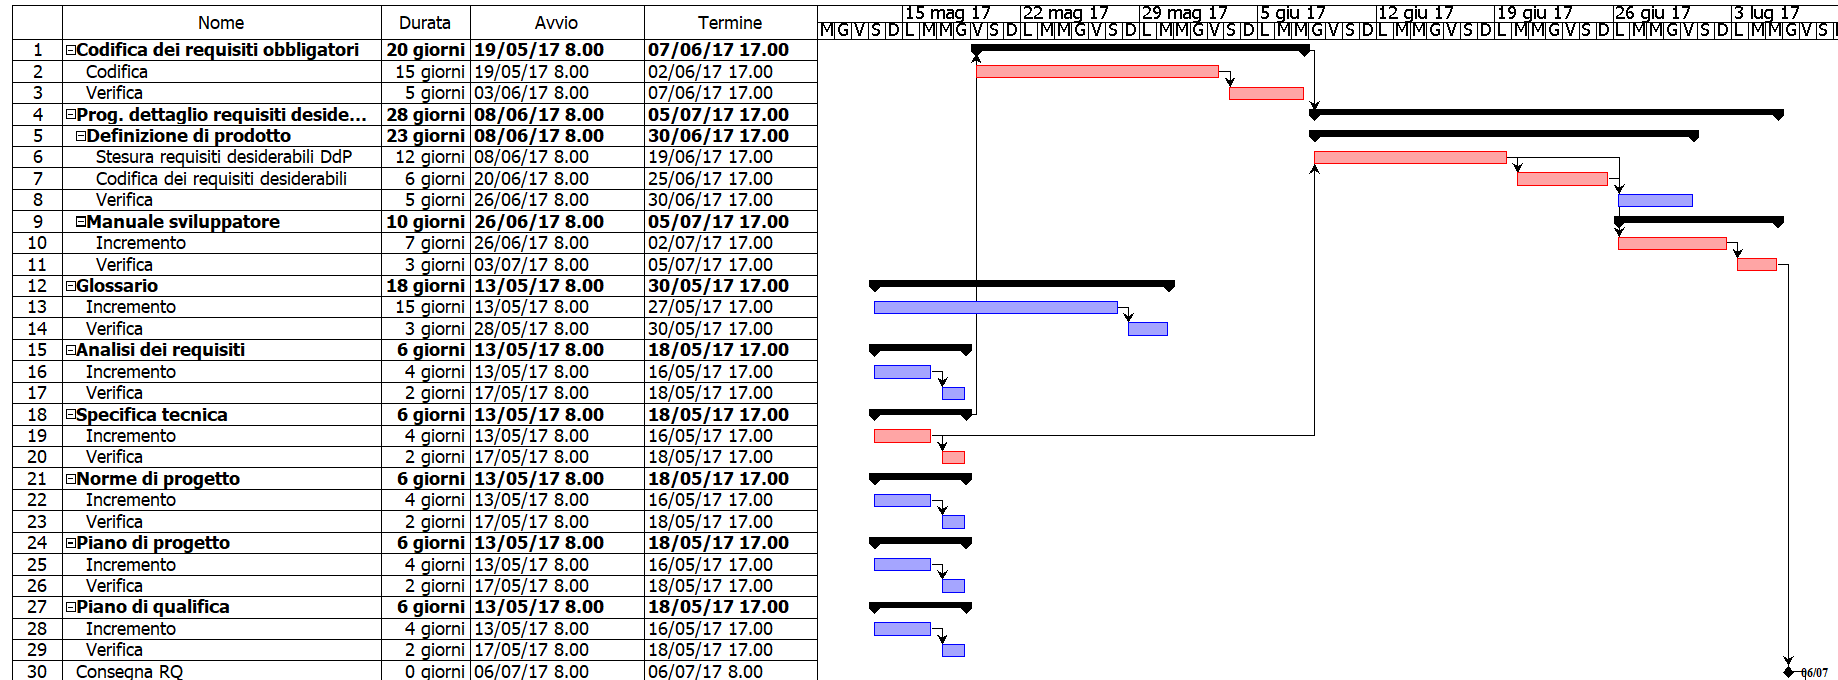
\includegraphics[scale=0.32]{Figures/toRQ}
		\caption{Periodo pre-RQ: Diagramma di Gantt}
	\end{figure}

	\subsubsection{Consuntivo di periodo}
	\begin{table}[H]
		\center
		\begin{tabularx}{\textwidth}{XXX}
			\noalign{\hrule height 1.5pt}
			\textbf{Ruolo} & \textbf{Ore} & \textbf{Costo(\euro)} \\
			\noalign{\hrule height 1.5pt}
			Responsabile &  12(0) & 360,00 (0,00) \\
			Amministratore &  17(0) & 340,00 (0,00) \\
			Analista &  24(0) & 600,00 (0,00) \\
			Progettista &  91(-8) & 2002,00 (-176,00)  \\
			Programmatore & 105(+16) & 1575,00(+240,00) \\
			Verificatore & 87(0) & 1305,00 (0,00) \\			
			\noalign{\hrule height 1.5pt}
			\textbf{Tot. consuntivo} & \textbf{336} & \textbf{6182,00} \\
			\textbf{Tot. preventivo} & \textbf{328} & \textbf{6118,00}\\
			\textbf{Differenza totali} & \textbf{+8} & \textbf{+64,00} \\
			\noalign{\hrule height 1.5pt}
		\end{tabularx}
		\caption{Consuntivo progettazione di dettaglio e codifica. \label{tab:table_label}}
	\end{table}
	
	\subsubsection{Conclusioni}
	Per questo periodo sono state risparmiate 5 ore per le attività dei \progettisti, dovuto ad una progettazione più dettagliata del previsto svolta nel periodo di Progettazione Architetturale; la maggior parte delle componenti del sistema sono state individuate nel periodo precedente. \\
	Inoltre sono state necessarie, per le attività dei \programmatori, 16 ore in più rispetto a quanto si è inizialmente preventivato; A queste si sono aggiunte 20 ore di autoformazione in più rispetto a quanto previsto, non riportate in tabella in quanto non a carico del committente. \\
	Il saldo tra consuntivo e preventivo è di \euro 64,00.
	
	
	\subsubsection{Preventivo a finire}
	Da quanto riportato nel precedente consuntivo si evince anche la necessità di una migliore stima delle ore necessarie ai vari ruoli, avendo constatato che sono necessarie un minore numero di ore per le attività dei \progettisti\ ed un numero maggiore di ore per le attività dei \programmatori. \\ 
	Date le precedenti sovrastime a preventivo il bilancio totale resta minore delle attese, i ritardi - legati a correzioni di errori o errata valutazione dei tempi necessari all'autoformazione e pertanto non a carico del committente - portano però il gruppo a dover rivedere la schedulazione prevista per il periodo che porterà alla \revisionediaccettazione. Si riporta il diagramma di Gantt relativo alla pianificazione aggiornata. \\
	\begin{figure}[H]
		\centering
		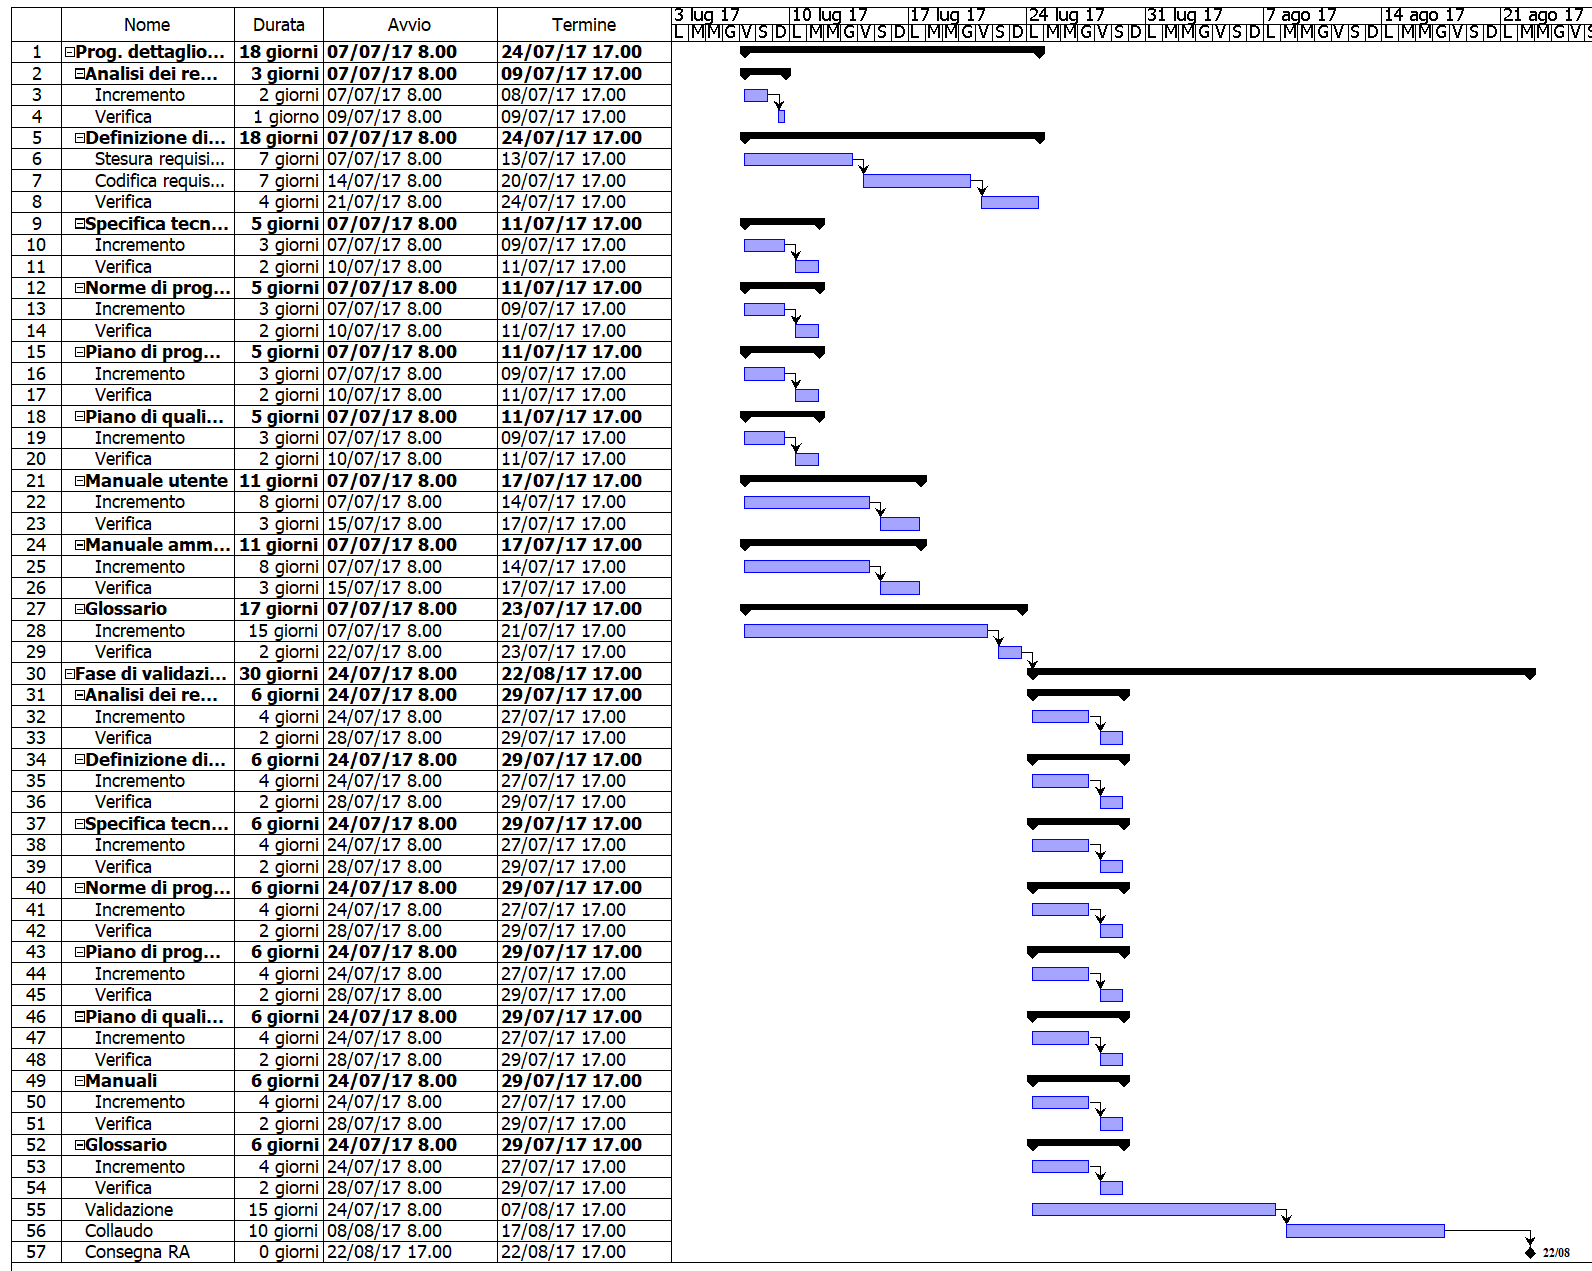
\includegraphics[scale=0.37]{Figures/RQtoRA}
		\caption{Periodo pre-RA: Diagramma di Gantt}
	\end{figure}
	Di seguito viene riportato il nuovo preventivo per le ore rendicontate; esso esclude i periodi di Analisi dei Requisiti e Analisi di dettaglio, che sono da intendere come investimento personale del gruppo \kaleidoscode. Alla luce di questo, il totale risultante \textbf{è a carico del committente}.
	
	
		\begin{table}[H]
		\center
		\begin{tabularx}{\textwidth}{XXX}
			\noalign{\hrule height 1.5pt}
			\textbf{Ruolo} & \textbf{Ore} & \textbf{Costo(\euro)} \\
			\noalign{\hrule height 1.5pt}
			Responsabile &  32(0) & 960,00 (0,00) \\
			Amministratore &  48(0) & 960,00 (0,00) \\
			Analista &  85(-4) & 2125,00 (-100,00) \\
			Progettista &  155(-12) & 3410,00 (-264,00)  \\
			Programmatore & 124(+16) & 1860,00(+240,00) \\
			Verificatore & 182(+4) & 2730,00 (+60,00) \\			
			\noalign{\hrule height 1.5pt}
			\textbf{Tot. preventivo} & \textbf{626} & \textbf{12045,00}\\
			\textbf{Differenza totali} & \textbf{+4} & \textbf{-64,00} \\
			\noalign{\hrule height 1.5pt}
		\end{tabularx}
		\caption{Tabella ore e costo totale. \label{tab:table_label}}
	\end{table}
		
\end{document}
